%!TEX program = xelatex

\documentclass[compress]{beamer}
%--------------------------------------------------------------------------
% Common packages
%--------------------------------------------------------------------------

\definecolor{links}{HTML}{663000}
\hypersetup{colorlinks,linkcolor=,urlcolor=links}

\usepackage[english]{babel}
\usepackage{pgfpages} % required for notes on second screen
\usepackage{graphicx}

\usepackage{multicol}


\usepackage{tabularx,ragged2e}
\usepackage{booktabs}

\setlength{\emergencystretch}{3em}  % prevent overfull lines
\providecommand{\tightlist}{%
  \setlength{\itemsep}{0pt}\setlength{\parskip}{0pt}}


\usetheme{hri}

\usepackage{remreset}% tiny package containing just the \@removefromreset command
\makeatletter
\@removefromreset{subsection}{section}
\makeatother
\setcounter{subsection}{1}

\makeatletter
\let\beamer@writeslidentry@miniframeson=\beamer@writeslidentry
\def\beamer@writeslidentry@miniframesoff{%
  \expandafter\beamer@ifempty\expandafter{\beamer@framestartpage}{}% does not happen normally
  {%else
    % removed \addtocontents commands
    \clearpage\beamer@notesactions%
  }
}
\newcommand*{\miniframeson}{\let\beamer@writeslidentry=\beamer@writeslidentry@miniframeson}
\newcommand*{\miniframesoff}{\let\beamer@writeslidentry=\beamer@writeslidentry@miniframesoff}
\makeatother


\newcommand{\source}[2]{{\tiny\it Source: \href{#1}{#2}}}

\usepackage{tikz}
\usetikzlibrary{mindmap,backgrounds,positioning}

\graphicspath{{figs/}}

\title{hacker\_space}
\subtitle{let's start hacking}
\date{}
\author{Séverin Lemaignan}
\institute{Bristol Robotics Lab\\{\bf University of the West of
England/University of Bristol}}

\begin{document}

%\licenseframe{github.com/severin-lemaignan/module-introduction-sensors-actuators}

\maketitle


\begin{frame}{Who am I?}

\begin{center}
    \textbf{Séverin Lemaignan} / \url{severin.lemaignan@brl.ac.uk}
\end{center}

\begin{multicols}{2}

    \textbf{Senior Researcher}@BRL

    \textbf{Cognitive robotics}

  Building robots and their artificial intelligence inspired on natural
  systems, such as developing children

    \textbf{Human-Robot Interaction}

  Building robots that can work alongside people, using social cues that
  people use to communicate

    \begin{center}
        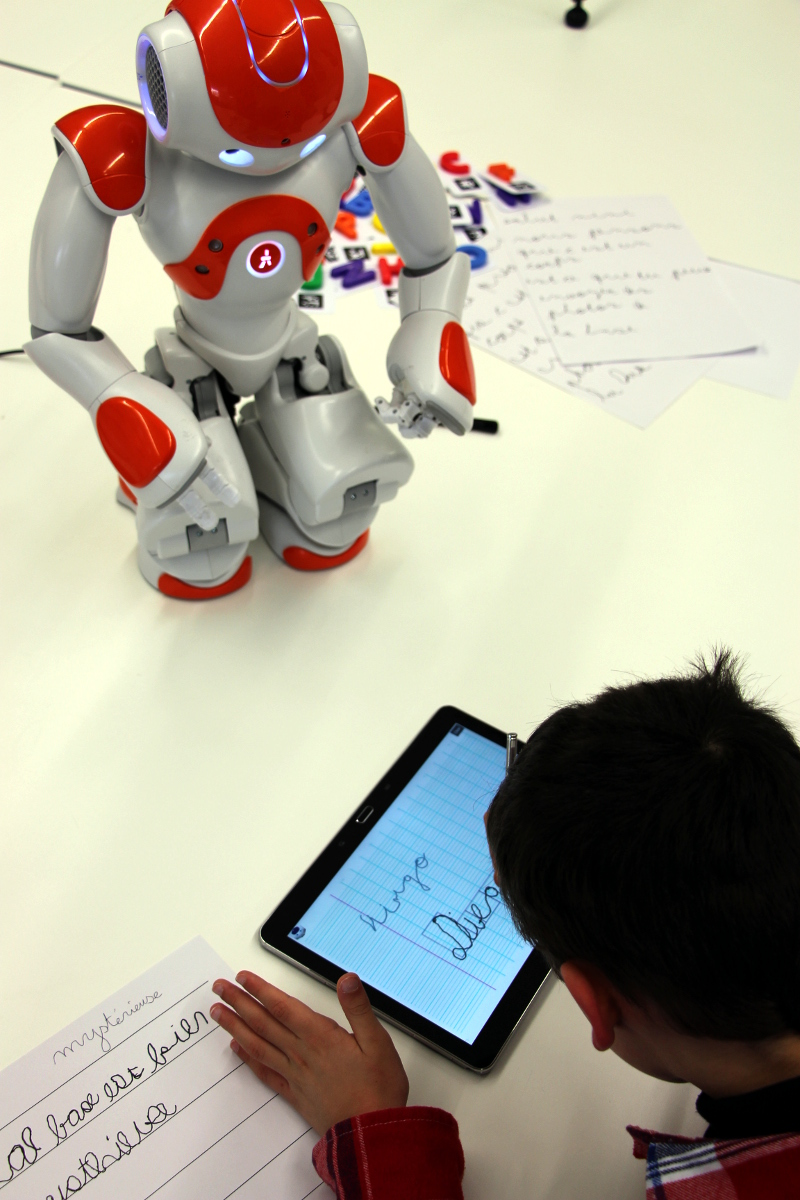
\includegraphics[width=0.7\linewidth]{cowriter}
    \end{center}

\end{multicols}
\end{frame}
%\begin{frame}[plain]
%    \begin{center}
%        \Large
%        \href{https://www.mentimeter.com/s/3ca728c0780550ff7296e7c31af2e317/b90ca40dfa36}{Go
%        to www.menti.com and use the code 15 14 87}
%    \end{center}
%\end{frame}

\section[hacker\_space]{BRL's hacker\_space}

\imageframe[color=black]{hacker_space}


\begin{frame}{BRL's hacker\_space}

    \begin{itemize}
        \item<1-> \textbf{open 24/7 for you}
        \item<2-> lockers where to leave your projects
        \item<3-> dual-boot computers (with CAD software)
        \item<3-> soldering stations, scopes, basic tools
    \end{itemize}

\end{frame}

\imageframe[caption=Loads of kits]{raspi-arduino}
\imageframe[caption=Loads of kits]{components}

\begin{frame}{During work hours...}
    \begin{itemize}
        \item Julian \& Josh are around
        \item Access to the hacker\_space workshop (press drill, etc)
        \item Access to the kits (you need to sign them out per project)
    \end{itemize}
    \pause

    \centering
    \bf
    I'll be around every Wednesday afternoon as well, 2pm-5pm, for support with your projects
\end{frame}

\imageframe[color=black]{hacker_space_workshop}

\begin{frame}{Exclusive membership card}
    \begin{center}
        \includegraphics<1>[width=0.8\linewidth]{media/member_card}
        \includegraphics<2>[width=0.8\linewidth]{media/member_card_achievements}
        \only<3>{(I've heard of a mythical 'golden card'...)}
    \end{center}
\end{frame}

\begin{frame}[plain]{}
    \centering
    \Large
    And if needed...
\end{frame}


\imageframe[color=black]{brl_workshop}
\imageframe[color=black]{brl_rp}


\section{A space for thinkering with crazy ideas}

\videoframe[0.56]{figs/projects/ROCO222-Robot-Arm-1st-demo-.3gpp.mp4}
\imageframe[color=black]{figs/projects/auto_maze}
\videoframe[0.56]{figs/projects/Gesture-controlled-Drone.3gpp.mp4}
\imageframe[color=black]{figs/projects/FinalMotor}
\imageframe[color=black]{figs/projects/3d_scanner}
\videoframe[0.56]{figs/projects/pothole_detection.webm}
\imageframe[color=black]{figs/projects/haptic_obstacle_detector}
\videoframe[0.56]{figs/projects/3D-printed-Robot-Arm-controlled-with-ROS.3gpp.mp4}
\videoframe[1.4]{figs/projects/IMU_RC_Car.mp4}
\videoframe[0.56]{figs/projects/gun_turret.mov}


\videoframe[0.56]{figs/NISSAN-ProPILOT-chair.mp4}

\begin{frame}[plain]{}
    \centering
    \Large
    Or maybe...
\end{frame}

\imageframe[color=black]{robotcup}
\imageframe[color=black]{eurobot}

\begin{frame}{On top of that...}
    \begin{itemize}
        \item<+-> Targeted tutorials on stuff you might not have in the main
            curriculum (Linux 101, C++ programming/compiling, GIT + GitHub, ROS
            the
            Robot Operating System...)

        \item<+-> Interactions with the incubator's start-ups

        \item<+-> hacker\_space competitions/challenges/open day events? up to
            you!

    
    \end{itemize}
\end{frame}


\begin{frame}{BRL's hacker\_space}

    \begin{center}
        
\includegraphics[width=0.4\linewidth]{needyou}

        \Large

        This is \emph{your} space:

        \textbf{Make it your own!!}

        \onslide<2>
        I'm looking for student reps for the hacker\_space!
    \end{center}
    

\end{frame}

\begin{frame}[plain]


        \Large

        {\bf
        On 4th Decemberi at 12pm:\\        
        Launch event with free pizza
        }

        \pause
        See you on Wednesday, 2pm!


\end{frame}


\end{document}
